% Source: src-b19b233abb266d1b051ded3c332a399c1722d8192d07ce1bf2234dda57bd25bc, PDF p.2.
% Right triangular prism topology and the specified line BC_1; schematic projection.
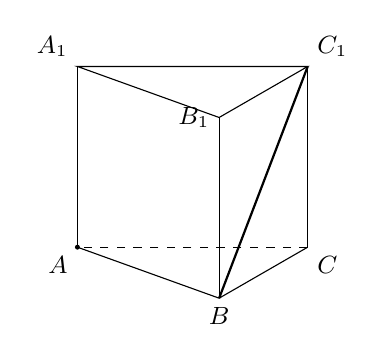
\begin{tikzpicture}[scale=0.9, every node/.style={font=\small}]
  \coordinate (A) at (0,0);
  \coordinate (B) at (2.0,-0.72);
  \coordinate (C) at (3.25,0);
  \coordinate (A1) at (0,2.55);
  \coordinate (B1) at (2.0,1.83);
  \coordinate (C1) at (3.25,2.55);
  \draw (A)--(B)--(C);
  \draw[dashed] (C)--(A);
  \draw (A1)--(B1)--(C1)--cycle;
  \draw (A)--(A1) (B)--(B1) (C)--(C1);
  \draw[thick] (B)--(C1);
  \fill (A) circle (1pt);
  \node[below left] at (A) {$A$};
  \node[below] at (B) {$B$};
  \node[below right] at (C) {$C$};
  \node[above left] at (A1) {$A_1$};
  \node[left] at (B1) {$B_1$};
  \node[above right] at (C1) {$C_1$};
\end{tikzpicture}
